%%
% This is an Overleaf template for presentations
% using the TUM Corporate Desing https://www.tum.de/cd
%
% For further details on how to use the template, take a look at our
% GitLab repository and browse through our test documents
% https://gitlab.lrz.de/latex4ei/tum-templates.
%
% The tumbeamer class is based on the beamer class.
% If you need further customization please consult the beamer class guide
% https://ctan.org/pkg/beamer.
% Additional class options are passed down to the base class.
%
% If you encounter any bugs or undesired behaviour, please raise an issue
% in our GitLab repository
% https://gitlab.lrz.de/latex4ei/tum-templates/issues
% and provide a description and minimal working example of your problem.
%%

\documentclass[
  german,            % define the document language (english, german)
  aspectratio=169,    % define the aspect ratio (169, 43)
  % handout=2on1,       % create handout with multiple slides (2on1, 4on1)
  % partpage=false,     % insert page at beginning of parts (true, false)
  % sectionpage=true,   % insert page at beginning of sections (true, false)
]{tumbeamer}


% load additional packages
\usepackage{booktabs}
\usepackage{graphicx}
\usepackage{tikz}
\usepackage{url}
\usepackage{pgfplots}
\usepackage{hyperref}
\usepackage{pmboxdraw}
\usepackage{float}
\usepackage{babel}[ngerman]
\usepackage{csquotes}[autostyle]
\usepackage[useregional]{datetime2}
\usepackage{listings}
\usepackage{xurl}
\usetikzlibrary{patterns}


\lstset {
    frame=single,
    tabsize=4,
    breaklines=true,
    xleftmargin=5pt,
    xrightmargin=5pt,
    basicstyle=\ttfamily\footnotesize,
    %language=[RISC-V]Assembler,
}

\hypersetup { 
  colorlinks=true,
  urlcolor=blue,
  filecolor=black,
  linkcolor=black
}

% tikz  
\usetikzlibrary{fit}

% image path
\graphicspath{ {../resources/} }

% presentation metadata
\title{Übung 04: Rekursion \& Calling Convention}
\subtitle{Einführung in die Rechnerarchitektur}
\author{\theAuthorName}

\institute{\theGroupName\\\theSchoolName\\\theUniversityName}
\date{11. -- \DTMdisplaydate{2024}{11}{17}{-1}}

\footline{\insertauthor~|~\insertshorttitle~|~\insertshortdate}


% macro to configure the style of the presentation
\TUMbeamersetup{
  title page = TUM tower,         % style of the title page
  part page = TUM toc,            % style of part pages
  section page = TUM toc,         % style of section pages
  content page = TUM more space,  % style of normal content pages
  tower scale = 1.0,              % scaling factor of TUM tower (if used)
  headline = TUM threeliner,      % which variation of headline to use
  footline = TUM default,         % which variation of footline to use
  % configure on which pages headlines and footlines should be printed
  headline on = {title page},
  footline on = {every page, title page=false},
}


% available frame styles for title page, part page, and section page:
% TUM default, TUM tower, TUM centered,
% TUM blue default, TUM blue tower, TUM blue centered,
% TUM shaded default, TUM shaded tower, TUM shaded centered,
% TUM flags
%
% additional frame styles for part page and section page:
% TUM toc
%
% available frame styles for content pages:
% TUM default, TUM more space
%
% available headline options:
% TUM empty, TUM oneliner, TUM twoliner, TUM threeliner, TUM logothreeliner
%
% available footline options:
% TUM empty, TUM default, TUM infoline


\begin{document}

\maketitle

\begin{frame}[c]{Mitschriften \& Infos}{}
  \begin{minipage}[t]{\textwidth}
    \begin{columns}[c]
      \begin{column}{0.8\textwidth}
        Montags: \href{\zulipMo}{\zulipMo}
      \end{column}
      \begin{column}{0.2\textwidth}
        \includegraphics[width=0.8\linewidth]{\zulipMoQrFilename}
      \end{column}
    \end{columns}
  \end{minipage}
  \rule{\textwidth}{0.4pt}
  \begin{minipage}[t]{\textwidth}
    \begin{columns}[c]
      \begin{column}{0.8\textwidth}
        Donnerstags: \href{\zulipDo}{\zulipDo}
      \end{column}
      \begin{column}{0.2\textwidth}
        \includegraphics[width=0.8\linewidth]{\zulipDoQrFilename}
      \end{column}
    \end{columns}
  \end{minipage}
  \ifdefined\myWebsite
  \rule{\textwidth}{0.4pt}
  \centering
  Website: \href{\myWebsite}{\myWebsite}
  \fi
\end{frame}

\begin{frame}[c]{}{}
  \begin{center}
    \LARGE  Keine Garantie für die Richtigkeit der Tutorfolien.

    \Large Bei Unklarheiten/Unstimmigkeiten haben VL/ZÜ-Folien recht!
  \end{center}
\end{frame}

\begin{frame}[c]{Inhaltsübersicht}{}
  \begin{columns}[c]
    \begin{column}{1\textwidth}
      \begin{itemize}
        \item Wiederholung
        \item Tutorblatt
        \begin{itemize}
          \item Calling Convention
          \item Rekursion in der Theorie
          \item Größter gemeinsamer Teiler
        \end{itemize}
      \end{itemize}
    \end{column}
  \end{columns}
\end{frame}

\begin{frame}[c]{Calling Convention}
  \begin{columns}[c]
    \begin{column}{0.5\textwidth}
      \begin{itemize}
        \item ``Vertrag`` zwischen allen Entwicklern
        \item Unterteilung von Register in Caller und Callee saved
        \begin{itemize}
          \item Caller saved Register dürfen direkt verändert werden
          \item Callee saved Register bleiben über Unterprogrammaufrufe erhalten
        \end{itemize} 
        \item \url{https://www.moodle.tum.de/mod/resource/view.php?id=3219780}
      \end{itemize}
    \end{column}
    \begin{column}{0.5\textwidth}
      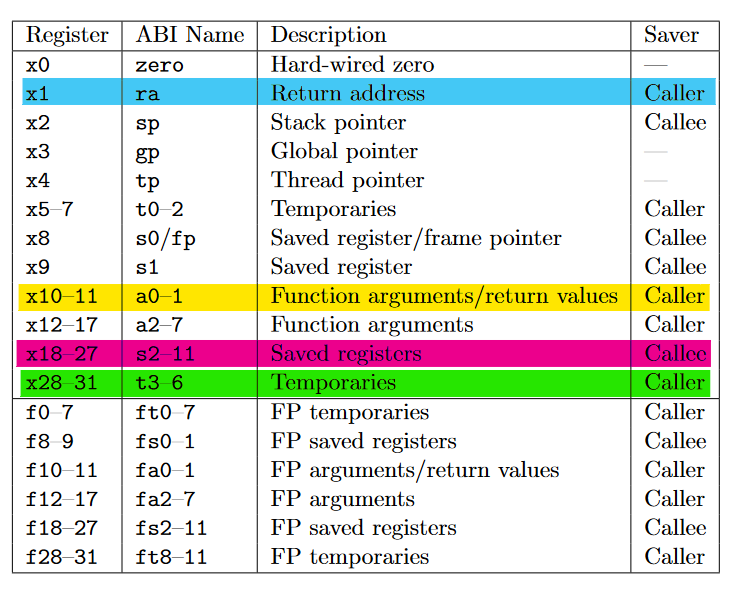
\includegraphics[width=\linewidth]{w03_calling_conv_regs.png}
    \end{column}
  \end{columns}
\end{frame}

\begin{frame}[c]{Calling Convention}                                    
  \begin{itemize}
    \item Datentypen kleiner als 32-Bit werden auf 32-Bit Sign-extended
    \item 64-Bit Werte in zwei a-Registern pro Wert, aufsteigend sortiert, untere Bit in niedrigerem Register
    \item >64 Bit werden als Pointer übergeben
    \item Weitere Parameter werden über den Stack übergeben
    \item Stack muss immer 16-Byte aligned sein
 \end{itemize}                                          
\end{frame}

\begin{frame}[c, fragile]{Rekursion}{}
  \begin{itemize}
    \item Funktion die \textbf{sich selbst aufruft}
    \item Viele Probleme haben rekursive Struktur, dadurch ist Rekursion häufig intuitiv
  \end{itemize}
  \begin{columns}[c]
    \begin{column}{0.48\textwidth}
      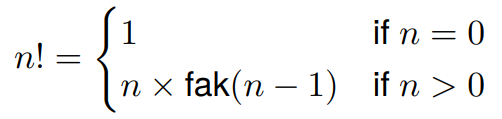
\includegraphics[width=0.9\linewidth]{w04_fak_rec_zue.png}
    \end{column}
    \begin{column}{0.48\textwidth}
      z.B. \\
      1! = 1 \\
      5! = 5 * 4 * 3 * 2 * 1 = 120
    \end{column}
  \end{columns}
  \begin{columns}[c]
    \begin{column}{0.48\textwidth}
      \begin{lstlisting}[
        basicstyle=\ttfamily,
        numbers=left,
        stepnumber=1,
        showstringspaces=false,
        tabsize=1,
        breaklines=true,
        breakatwhitespace=false,
        frame=single,
      ]
int f(int n) {
  if (n==0 || n==1)
    return 1;
  return n*f(n-1);
}
      \end{lstlisting}
      \centering
      (rekrusiv)
    \end{column}
    \begin{column}{0.48\textwidth}
      \begin{lstlisting}[
        basicstyle=\ttfamily,
        numbers=left,
        stepnumber=1,
        showstringspaces=false,
        tabsize=1,
        breaklines=true,
        breakatwhitespace=false,
        frame=single,
      ]
int f(int n) {
  int a = 1;
  for(int i=0; i<=n; i++)
    a = a * i;
  return a;
}
      \end{lstlisting}
      \centering
      (iterativ)
    \end{column}
  \end{columns}
\end{frame}

\begin{frame}[c, fragile]{Rekursion: Schema}{}
  \begin{enumerate}
    \item Basisfall (Abbruchbedingung) prüfen
      \begin{itemize}
        \item Wenn ja --> vordefinierten Wert zurückgeben
        \item Wenn nein --> weiter mit rekursiver Berechnung
      \end{itemize}
    \item Sicherung von \verb|ra| und evtl. Parametern
    \item Vorbereitung der Parameter für den rekursiven Aufruf
    \item Rekursiver Aufruf
    \item Ergebnis des Aufrufs verwerten
    \item Wiederherstellung von \verb|ra|, \verb|sp|
    \item Rücksprung
  \end{enumerate}
\end{frame}

\begin{frame}[c, fragile]{Rekursion: Beispiel}{}
  \begin{columns}[c]
    \begin{column}{0.4\textwidth}
      \begin{lstlisting}[
        basicstyle=\ttfamily,
        numbers=left,
        stepnumber=1,
        showstringspaces=false,
        tabsize=4,
        breaklines=true,
        breakatwhitespace=false,
        frame=single,
      ]
fun:
  addi sp, sp, -8
  sw ra, 0(sp)
  sw a0, 4(sp)
  beq a0, zero, end
  addi a0, a0, -1
  jal fun
  end:
  lw ra, 0(sp)
  addi sp, sp, 8
  jalr zero, 0(ra)
      \end{lstlisting}
      \small \textbf{Achtung}: 8 Byte nicht CC-konform, nur zur besseren Darstellung
    \end{column}
    \begin{column}{0.5\textwidth}
      Aufruf mit {\ttfamily a0 = 3}:
      \vspace{2cm}
    \end{column}
  \end{columns}
\end{frame}


\begin{frame}[c, fragile]{Rekursion: Beispiel}{}
  \begin{columns}[c]
    \begin{column}{0.4\textwidth}
      \begin{lstlisting}[
        basicstyle=\ttfamily,
        numbers=left,
        stepnumber=1,
        showstringspaces=false,
        tabsize=4,
        breaklines=true,
        breakatwhitespace=false,
        frame=single,
      ]
fun:
  addi sp, sp, -8
  sw ra, 0(sp)
  sw a0, 4(sp)
  beq a0, zero, end
  addi a0, a0, -1
  jal fun
  end:
  lw ra, 0(sp)
  addi sp, sp, 8
  jalr zero, 0(ra)
      \end{lstlisting}
      \small \textbf{Achtung}: 8 Byte nicht CC-konform, nur zur besseren Darstellung
    \end{column}
    \begin{column}{0.5\textwidth}
      Aufruf mit {\ttfamily a0 = 3}:
      \begin{center}
        \begin{tikzpicture}[scale=0.8]
          \def\stackwidth{2.5}
          \def\stackheight{0.6}
          \def\cellheight{0.6}
          \def\cellwidth{2.5}

          \foreach \slide/\vala/\valb in {1/0x3/ra, 2/0x2/ra, 3/0x1/ra, 4/0x0/ra} {
              \only<\slide->{
                \draw (0,-\slide*2*\stackheight+\stackheight) rectangle ++(\stackwidth, -\cellheight) node[midway] {\texttt{\vala}};
                \draw (0,-\slide*2*\stackheight) rectangle ++(\stackwidth, -\cellheight) node[midway] {\texttt{\valb}};
              }
              \only<\slide>{
                \draw[<-, ultra thick] (\stackwidth+0.2, -\slide*2*\stackheight-\stackheight) -- ++(1,0) node [right] {\ttfamily{sp}};
              }
            }

          \foreach \x/\vala/\valb in {1/ffff/fffb, 2/fff7/fff3, 3/ffef/ffeb, 4/ffe7/ffe3} {
            \only<\x->{
              \node[anchor=east] at (-0.2, -\x*2*\stackheight+\stackheight - \cellheight/2) {\texttt{0x\vala}};
              \node[anchor=east] at (-0.2, -\x*2*\stackheight - \cellheight/2) {\texttt{0x\valb}};
            }
            } 

          \foreach \slide/\y in {5/2, 6/4, 7/6, 8/8}{
              \only<\slide>{
                \draw[pattern=north east lines, pattern color=red] (0,-9*\stackheight) rectangle ++(\stackwidth, \y*\stackheight);
                \draw[<-, ultra thick] (\stackwidth+0.2, \y*\stackheight-9*\stackheight) -- ++(1,0) node [right] {\ttfamily{sp}};
              }
            }
        \end{tikzpicture}
      \end{center}
    \end{column}
  \end{columns}
\end{frame}


\begin{frame}[c]{}{}
  \begin{center}
    \LARGE Fragen?
  \end{center}
  \vspace{0.5cm}
  \begin{center}
    \LARGE Bis zum nächsten Mal ;) \\
  \end{center}
  \vspace{1.0cm}
  \begin{center}
    \small Folien inspiriert von Niklas Ladurner
  \end{center}
\end{frame}

\end{document}